\documentclass[french,]{article}
\usepackage{lmodern}
\usepackage{amssymb,amsmath}
\usepackage{ifxetex,ifluatex}
\usepackage{fixltx2e} % provides \textsubscript
\ifnum 0\ifxetex 1\fi\ifluatex 1\fi=0 % if pdftex
  \usepackage[T1]{fontenc}
  \usepackage[utf8]{inputenc}
\else % if luatex or xelatex
  \ifxetex
    \usepackage{mathspec}
  \else
    \usepackage{fontspec}
  \fi
  \defaultfontfeatures{Ligatures=TeX,Scale=MatchLowercase}
\fi
% use upquote if available, for straight quotes in verbatim environments
\IfFileExists{upquote.sty}{\usepackage{upquote}}{}
% use microtype if available
\IfFileExists{microtype.sty}{%
\usepackage{microtype}
\UseMicrotypeSet[protrusion]{basicmath} % disable protrusion for tt fonts
}{}
\usepackage[top=2cm,bottom=2cm]{geometry}
\usepackage{hyperref}
\hypersetup{unicode=true,
            pdfborder={0 0 0},
            breaklinks=true}
\urlstyle{same}  % don't use monospace font for urls
\ifnum 0\ifxetex 1\fi\ifluatex 1\fi=0 % if pdftex
  \usepackage[shorthands=off,main=french]{babel}
\else
  \usepackage{polyglossia}
  \setmainlanguage[]{french}
\fi
\usepackage{longtable,booktabs}
\usepackage{graphicx,grffile}
\makeatletter
\def\maxwidth{\ifdim\Gin@nat@width>\linewidth\linewidth\else\Gin@nat@width\fi}
\def\maxheight{\ifdim\Gin@nat@height>\textheight\textheight\else\Gin@nat@height\fi}
\makeatother
% Scale images if necessary, so that they will not overflow the page
% margins by default, and it is still possible to overwrite the defaults
% using explicit options in \includegraphics[width, height, ...]{}
\setkeys{Gin}{width=\maxwidth,height=\maxheight,keepaspectratio}
\IfFileExists{parskip.sty}{%
\usepackage{parskip}
}{% else
\setlength{\parindent}{0pt}
\setlength{\parskip}{6pt plus 2pt minus 1pt}
}
\setlength{\emergencystretch}{3em}  % prevent overfull lines
\providecommand{\tightlist}{%
  \setlength{\itemsep}{0pt}\setlength{\parskip}{0pt}}
\setcounter{secnumdepth}{0}
% Redefines (sub)paragraphs to behave more like sections
\ifx\paragraph\undefined\else
\let\oldparagraph\paragraph
\renewcommand{\paragraph}[1]{\oldparagraph{#1}\mbox{}}
\fi
\ifx\subparagraph\undefined\else
\let\oldsubparagraph\subparagraph
\renewcommand{\subparagraph}[1]{\oldsubparagraph{#1}\mbox{}}
\fi

%%% Use protect on footnotes to avoid problems with footnotes in titles
\let\rmarkdownfootnote\footnote%
\def\footnote{\protect\rmarkdownfootnote}

%%% Change title format to be more compact
\usepackage{titling}

% Create subtitle command for use in maketitle
\newcommand{\subtitle}[1]{
  \posttitle{
    \begin{center}\large#1\end{center}
    }
}

\setlength{\droptitle}{-2em}
  \title{}
  \pretitle{\vspace{\droptitle}}
  \posttitle{}
  \author{}
  \preauthor{}\postauthor{}
  \date{}
  \predate{}\postdate{}


\usepackage[utf8]{inputenc}
\usepackage[T1]{fontenc}
\usepackage[francais]{babel}
\usepackage{setspace}
\usepackage{soul}
\usepackage{ulem}
%usepackage{color}
\usepackage{url}
\usepackage[top=1.5cm, bottom=2.5cm, left=2cm, right=2cm]{geometry}
\usepackage{layout}
\usepackage{lmodern}
\usepackage{fancyhdr}
\usepackage{graphicx}
\usepackage{wrapfig}
\usepackage{multirow}
\usepackage{array}
\usepackage{eurosym}
\usepackage{xcolor}
\usepackage{colortbl}
\usepackage{amsmath}
\usepackage{amssymb}
\usepackage{mathrsfs}
\usepackage{makeidx}
\usepackage[absolute]{textpos}
\usepackage[cc]{titlepic}
\usepackage{booktabs}
\usepackage[table,xcdraw]{xcolor}
\usepackage{minitoc}
\usepackage{keyval}
\usepackage{epsfig}
\usepackage{chngpage}
\usepackage{tikz}
\usepackage{tkz-euclide}
\usetkzobj{all}
\usepackage[landscape]{geometry}
\usepackage{listings}
\usepackage{tabularx}
\usepackage{minted}

\usepackage{fancyvrb}

\onehalfspacing


%%%% debut macro %%%%
\newenvironment{changemargin}[1]{\begin{list}{}{%
\setlength{\topsep}{0pt}%
\setlength{\leftmargin}{0pt}%
\setlength{\rightmargin}{0pt}%
\setlength{\listparindent}{\parindent}%
\setlength{\itemindent}{\parindent}%
\setlength{\parsep}{0pt plus 1pt}%
\addtolength{\leftmargin}{#1}%
\addtolength{\rightmargin}{#2}%
}\item }{\end{list}}
%%%% fin macro %%%%

\definecolor{lightgray}{gray}{.90}


\begin{document}

\setlength{\parindent}{0cm}
\setlength{\parskip}{1ex plus 0.5ex minus 0.2ex}
\newcommand{\hsp}{\hspace{20pt}}
\newcommand{\HRule}{\rule{\linewidth}{0.5mm}}
\usetkzobj{all}

\begin{document}

\begin{titlepage}
  \begin{sffamily}
  \begin{center}

    \newcommand{\titreP}{Snake and Ladders game}
    \newcommand{\titreS}{Projet 1 - Markov Decision Processes}
    
    \includegraphics[scale=0.5]{EPLlogo.jpg}~\\[0.25cm]
    \textsc{\LARGE Ecole polytechnique de Louvain}\\[2cm]

    \textsc{\huge LSINF2275\\ Data Mining \& \\Decision Making}\\[1.5cm]

    % Title
    \HRule \\
    [0.4cm]
    {\huge \bfseries \titreP \\ \titreS \\
    [0.4cm] }
    \HRule \\
    [0.5cm]
    \begin{center}
            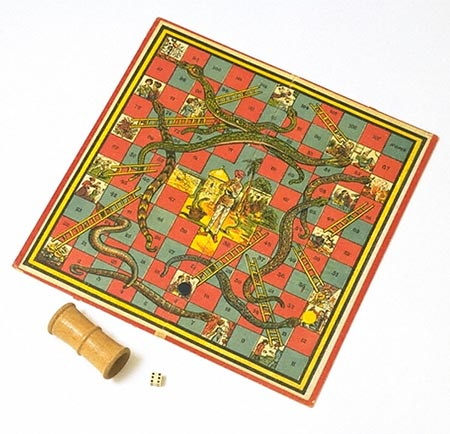
\includegraphics[scale=0.6]{snake_and_ladders.jpg}
    \end{center}

    % Author and supervisor
    \begin{minipage}{0.5\textwidth}
      \begin{flushleft} \large
        Guillaume  \textsc{TRUFFAUT } - noma - DATS2M\\ 
        Patrick \textsc{GUERIN} - 80541700 - DATS2M\\ 
     
       
      \end{flushleft}
    \end{minipage}
    \begin{minipage}{0.4\textwidth}
      \begin{flushright} \large
        Professeur :  Marco  \textsc{Saerens}\\
        \end{flushright}
    \end{minipage}

    \vfill

    % Bottom of the page
    {\today}

  \end{center}
  \end{sffamily}
\end{titlepage}

\graphicspath{ {(C:/Users/p/Documents/GitHub/markov-processes/} }

\newpage

`\tableofcontents'

\newpage

\section{1. Introduction et explication du
jeu}\label{introduction-et-explication-du-jeu}

L'objectif du projet est de mettre en application les processus de
décision markovien sur un jeu de l'oie. Ce dernier est modélisé de la
manière suivante :

\begin{figure}[h]
\caption{Schéma du jeu de l'oie modifié}
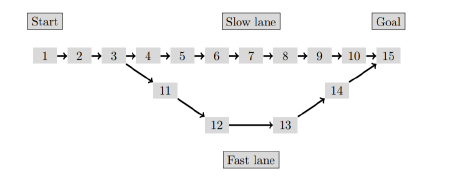
\includegraphics{jeu de l'oie.PNG}
\centering
\end{figure}

Pour commencer, nous avons initialisé le jeu avec deux pièges. Le
premier est situé sur la case 7 et le second sur la case 13. Le premier,
en cas d'activation, fait reculer le joueur de 3 cases jusqu'à la case
4. Le second piège, quant à lui, ramène le joueur à la case 1. Il est
important de préciser que le piège a une chance de s'activer dès que le
joueur arrive sur la case piégée. Exemple : Le joueur démarre de la case
5 et réalise un 2 en jouant le dé normal, il arrivera donc sur la case
7. Le joueur a, dès lors, une chance sur deux de rester sur la case 7 ou
de reculer de 3 cases. Cependant au prochain tour, le piège peut à
nouveau s'activer si le joueur réalise un 0 (sauf s'il a joué le dé de
sécurité).

Ensuite, le jeu sera joué selon deux règles différentes. La première
règle stipule que le joueur gagne le jeu dès qu'il (dé)passe la case 15.
La seconde règle qui est plus stricte exige à ce que le joueur arrive
exactement sur la case 15 pour gagner le jeu.

Pour la suite du projet, nous allons tout d'abord définir la stratégie
optimale à jouer selon la règle en vigueur (règle 1 ou règle 2) grâce
aux processus de decision markoviens. Ensuite nous simulerons
différentes parties afin de, tout d'abord, comparer les résultats
théoriques et empiriques de la stratégie optimale mais également de
comparer cette dernière avec d'autres stratégies qui seront normalement
moins efficaces (jouer toujours le même dé ou jouer aléatoirement).

\section{2. Théorie : algorithme d'itération de la
valeur}\label{theorie-algorithme-diteration-de-la-valeur}

Afin de trouver la stratégie optimale à jouer nous nous basons sur la
méthode de programmation dynamique de Richard Bellman. Le problème est
divisé en sous-problèmes: trouver la stratégie optimale pour chaque
case.

Ce jeu peut être vu comme un processus stochastique pour lequel le futur
est independant du passé, étant donné le présent. (propriété de Markov)

Autrement dit si \(X_{n}\) est la stratégie du joueur à la case n et
\(X_{n-1}\) la stratégie jouée à la case précédant n, on a alors:

\(\mathbb{P}(X_n=x_n\mid X_{n-1}=x_{n-1}, \dots, X_0=x_0)=\mathbb{P}(X_n=x_n\mid X_{n-1}=x_{n-1}).\)

\newpage

Pour résoudre ce processus de décision markovien, une ``politique'' de
jeu optimale peut ainsi être trouvée à l'aide de l'algorithme de la
``value iteration''. Ce dernier se base sur l'équation de Bellman pour
calculer de manière récursive le coût optimal esperé:

\[ \hat{V}(k) \leftarrow  \min_{a \in U_{k}} \bigg\{ c(a,k)+ \sum_{k'} p(k'|k,a) V^*(k')]\bigg\} \\ \hat{V}(d) \leftarrow0 , \text{où d est la case finale.}  \]

Avec :

\(\hat{V}(k)\) le coût attendu de la case k.

\(p(k'|k,a)\) la probabilité d'atteindre la case \(k'\) en jouant
l'action \(a\) depuis la case \(k\).

\(c(a,k)\) le coût de realisation de l'action a à la case k, ici 1 à
chaque fois.

L'action optimale a la case k est alors:

\[ {\arg\!\min}_{a \in U_{k}} \bigg\{ c(a,k)+ \sum_{k'} p(k'|k,a) V^*(k')]\bigg\} \]

\section{3. Simulation du jeu}\label{simulation-du-jeu}

Pour la simulation, afin d'obtenir des résultats précis, nous itérerons
chaque partie 10 000 fois. Ces dernières seront jouées selon 5
stratégies différentes :

\begin{itemize}
\tightlist
\item
  La stratégie optimale définie dans la partie 2 selon la règle jouée
\item
  Toujours le dé ``sécurité'' (dé 1)
\item
  Toujours le dé ``normal'' (dé 2)
\item
  Toujours le dé ``risqué'' (dé 3)
\item
  Stratégie définie de manière aléatoire
\end{itemize}

\newpage

\subsection{3.1 Simulation selon la règle
1}\label{simulation-selon-la-regle-1}

Nous allons tout d'abord jouer selon la règle 1 qui est dîte souple.
Ci-dessous, nous vous présentons les résultats des 10 000 parties jouées
selon les différentes stratégies. Pour chaque partie, nous la débutons à
partir de la case 1.

\begin{figure}[h]
\caption{Boxplots - Règle 1 }
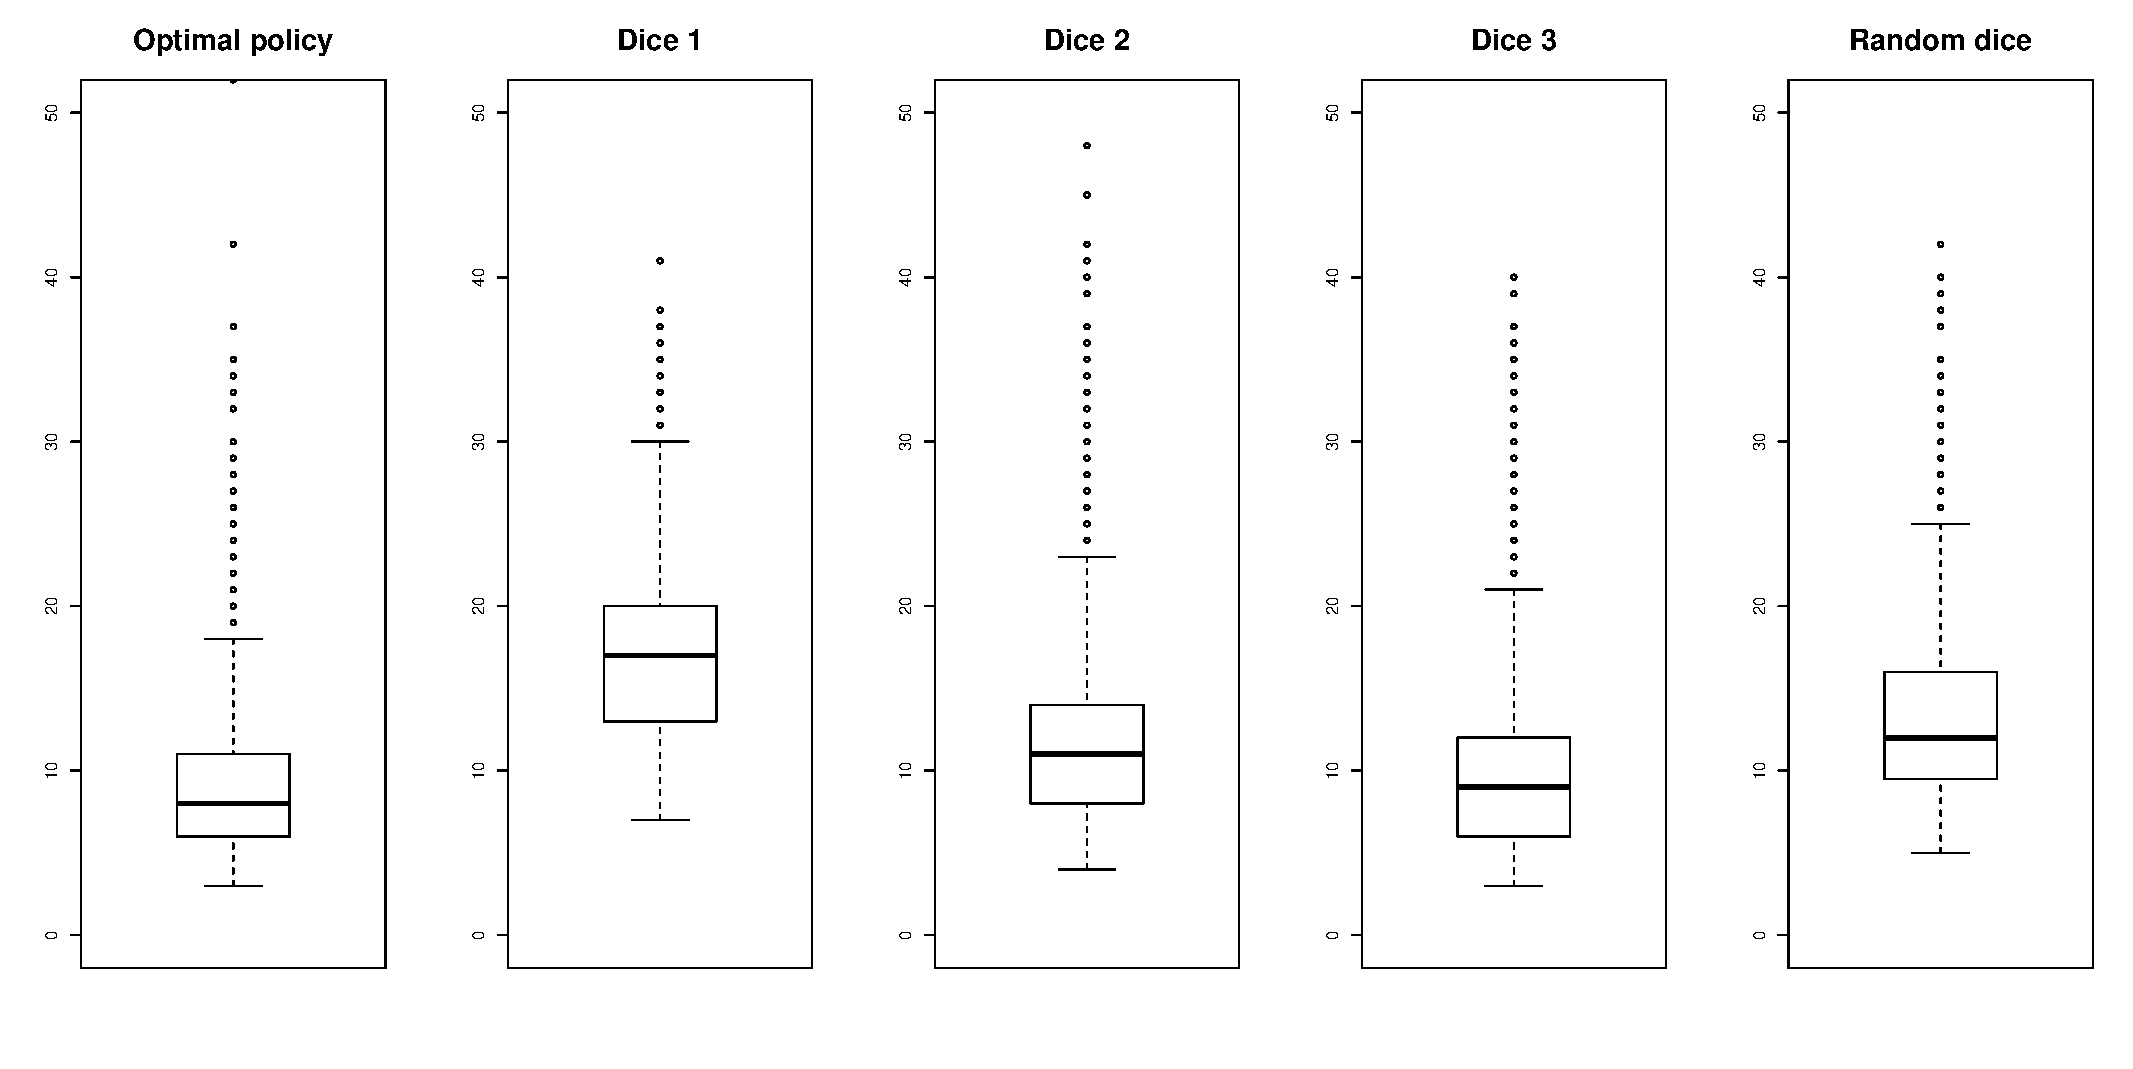
\includegraphics[height=10cm]{Boxplot_rule1.pdf}
\centering
\end{figure}

Nous pouvons déjà constater, qu'au départ de la case une, la stratégie
optimale a de meilleurs résultats en moyenne par rapport aux 4 autres
stratégies. La stratégie la moins efficace semble être celle qui joue
toujours le dé de sécurité. De manière intuitive, ce résultat est
cohérent car nous ne risquons pas de revenir aux premières cases lorsque
nous dépassons la case 15.

Ensuite, nous pouvons comparer les resultats des différentes stratégies
au départ de n'importe quelle case du jeu. Le tableau, ci-dessous vous
présente le nombre d'itérations moyen nécessaire pour terminer le jeu en
fonction de la case où le jeu a débuté.

\begin{longtable}[]{@{}lrrrrr@{}}
\caption{Nombre d'itérations moyen en fonction de la case de
départ}\tabularnewline
\toprule
& Optimal policy & Dice 1 & Dice 2 & Dice 3 & Random dice\tabularnewline
\midrule
\endfirsthead
\toprule
& Optimal policy & Dice 1 & Dice 2 & Dice 3 & Random dice\tabularnewline
\midrule
\endhead
Square 1 & 9.02 & 16.96 & 11.76 & 9.69 & 13.03\tabularnewline
Square 2 & 8.35 & 15.08 & 10.88 & 8.88 & 11.13\tabularnewline
Square 3 & 7.69 & 12.97 & 9.60 & 8.28 & 9.60\tabularnewline
Square 4 & 7.15 & 13.96 & 9.19 & 7.89 & 9.51\tabularnewline
Square 5 & 6.22 & 11.99 & 8.44 & 6.58 & 8.46\tabularnewline
Square 6 & 5.07 & 9.98 & 6.84 & 5.36 & 7.56\tabularnewline
Square 7 & 4.15 & 8.03 & 5.29 & 4.35 & 6.25\tabularnewline
Square 8 & 2.36 & 6.01 & 3.35 & 2.38 & 4.23\tabularnewline
Square 9 & 1.79 & 3.98 & 2.24 & 1.78 & 2.27\tabularnewline
Square 10 & 1.33 & 2.01 & 1.50 & 1.35 & 1.50\tabularnewline
Square 11 & 6.44 & 7.98 & 8.59 & 6.64 & 8.18\tabularnewline
Square 12 & 4.85 & 6.03 & 6.18 & 5.07 & 6.26\tabularnewline
Square 13 & 3.35 & 4.01 & 4.06 & 3.74 & 3.34\tabularnewline
Square 14 & 1.33 & 1.99 & 1.50 & 1.34 & 1.34\tabularnewline
\bottomrule
\end{longtable}

\newpage

Nous pouvons constater que la stratégie optimale est, en moyenne, soit
meilleure ou équivalente aux autres stratégies de jeu quelque soit la
case de départ. D'ailleurs, la stratégie de toujours jouer le dé risqué
est assez similaire à la stratégie optimale. Ceci n'est pas étonnant car
cette dernière préconise de jouer le dé risqué dans 12 cas sur 15.
Cependant, si nous analysons l'écart-type des resultats des différentes
stratégies, nous pouvons remarquer que la stratégie optimale fournit
bien un résultat moins variable que la stratégie du dé risqué.

\begin{longtable}[]{@{}lrrrrr@{}}
\caption{Variance des différentes stratégies}\tabularnewline
\toprule
& Optimal policy & Dice 1 & Dice 2 & Dice 3 & Random dice\tabularnewline
\midrule
\endfirsthead
\toprule
& Optimal policy & Dice 1 & Dice 2 & Dice 3 & Random dice\tabularnewline
\midrule
\endhead
Ecart-type & 4.12 & 5.12 & 5.24 & 4.83 & 4.84\tabularnewline
\bottomrule
\end{longtable}

\subsection{3.2 Simulation selon la règle
2}\label{simulation-selon-la-regle-2}

Nous allons maintenant changer la règle du jeu en obligeant le joueur de
tomber exactement sur la case 15 afin de remporter la partie.
Ci-dessous, retrouvez les résultats des differentes stratégies au départ
de la case 1.

\begin{figure}[h]
\caption{Boxplots - Règle 2 }
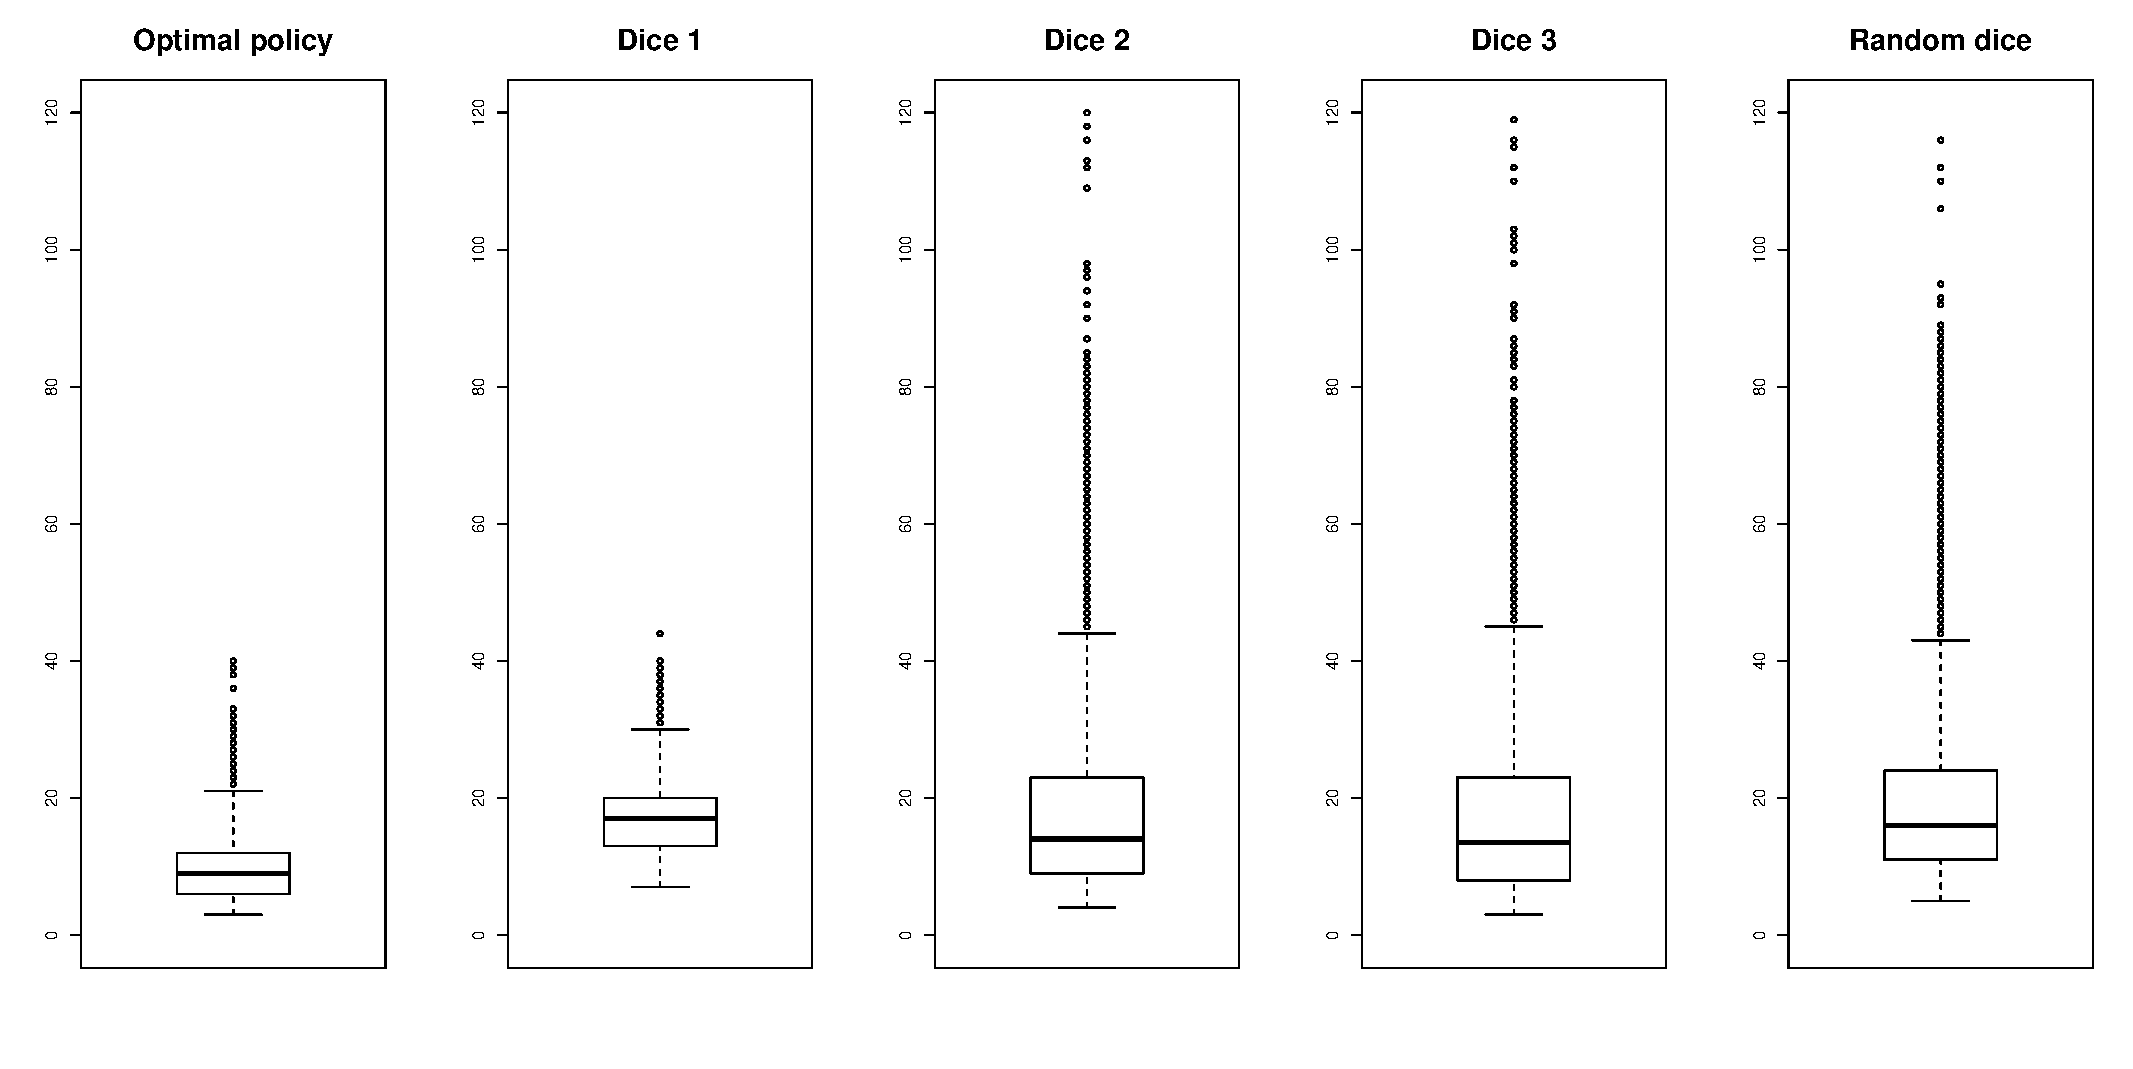
\includegraphics[height=8cm]{Boxplot_rule2.pdf}
\centering
\end{figure}

Selon la règle 2, jouer la stratégie optimale semble être plus efficace
que les 4 autres stratégies. Contrairement au cas de la règle 1, ici
c'est la stratégie du dé 1 qui semble se rapprocher de la stratégie
optimale. Ceci est cohérent du au fait que nous revenons aux cases de
départ si la case 15 est dépassée.

\newpage

Nous pouvons également analyser le résulat moyen au départ de n'importe
quelle case du jeu :

\begin{longtable}[]{@{}lrrrrr@{}}
\caption{Nombre d'itérations moyen en fonction de la case de
départ}\tabularnewline
\toprule
& Optimal policy & Dice 1 & Dice 2 & Dice 3 & Random dice\tabularnewline
\midrule
\endfirsthead
\toprule
& Optimal policy & Dice 1 & Dice 2 & Dice 3 & Random dice\tabularnewline
\midrule
\endhead
Square 1 & 9.52 & 17.05 & 18.32 & 17.64 & 19.08\tabularnewline
Square 2 & 8.91 & 15.09 & 17.54 & 16.70 & 17.23\tabularnewline
Square 3 & 8.07 & 12.97 & 16.49 & 15.99 & 16.92\tabularnewline
Square 4 & 7.67 & 14.03 & 15.62 & 15.90 & 14.52\tabularnewline
Square 5 & 6.79 & 12.02 & 14.84 & 14.38 & 13.36\tabularnewline
Square 6 & 5.64 & 10.00 & 13.16 & 13.61 & 12.53\tabularnewline
Square 7 & 4.72 & 8.00 & 11.23 & 13.41 & 11.10\tabularnewline
Square 8 & 2.84 & 6.02 & 10.30 & 9.32 & 8.99\tabularnewline
Square 9 & 2.52 & 4.00 & 6.78 & 11.66 & 7.25\tabularnewline
Square 10 & 1.98 & 2.00 & 10.70 & 12.80 & 11.05\tabularnewline
Square 11 & 6.93 & 8.00 & 15.71 & 15.27 & 17.95\tabularnewline
Square 12 & 5.24 & 5.99 & 13.81 & 11.58 & 16.71\tabularnewline
Square 13 & 3.93 & 4.00 & 9.16 & 12.83 & 15.46\tabularnewline
Square 14 & 2.01 & 2.01 & 10.99 & 12.84 & 13.31\tabularnewline
\bottomrule
\end{longtable}

En analysant en détail, il apparaît clairement, que pour toutes les
cases, la stratégie optimale est meilleure que n'importe quelle autre
stratégie sauf pour la case 14 avec la stratégie du dé 1. En effet, la
stratégie optimale préconise de jouer le dé sécurité pour l'avant
dernière case du jeu.

Nous pouvons également comparer l'indice de dispersion pour les
resultats des différentes stratégies :

\begin{longtable}[]{@{}lrrrrr@{}}
\caption{Variance des différentes stratégies}\tabularnewline
\toprule
& Optimal policy & Dice 1 & Dice 2 & Dice 3 & Random dice\tabularnewline
\midrule
\endfirsthead
\toprule
& Optimal policy & Dice 1 & Dice 2 & Dice 3 & Random dice\tabularnewline
\midrule
\endhead
Ecart-type & 4.33 & 5.17 & 13.11 & 14.09 & 12.13\tabularnewline
\bottomrule
\end{longtable}

En plus de présenter le meilleur résultat moyen, la stratégie optimale
est celle qui présente également une performance la moins variable dans
le contexte de la règle 2. Ceci confirme qu'elle est belle est bien la
plus éfficace.

\newpage

\section{4. Adaptation du jeu}\label{adaptation-du-jeu}

\section{4.1 Ajout d'un ralentisseur}\label{ajout-dun-ralentisseur}

Nous avons ensuite ajouté un piège en case 9 qui ralentit le joueur si
il est activé. Par exemple si le joueur arrive en case 9 et active le
piège, il avancera au tour suivant selon le chiffre tiré par son dé,
moins une case. Comme illustré ci-dessous, cela revient à ajouter une
case à notre jeu pour porter le nombre de cases à 16, si le piège est
activé le joueur fait un détour en case 10.

\begin{figure}[h]
\caption{Schéma conceptuel du jeu de l'oie avec un piège ralentisseur en case 9.}
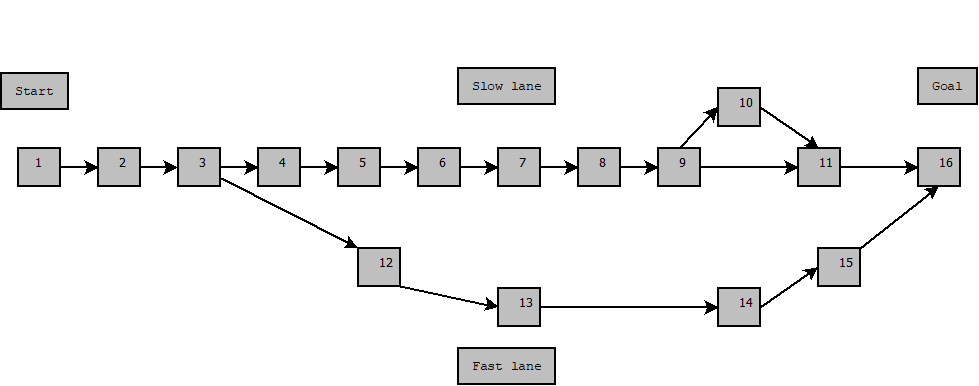
\includegraphics{schema2.PNG}
\end{figure}

\section{4.2 Analyses des différentes stratégies selon le plateau de
jeu}\label{analyses-des-differentes-strategies-selon-le-plateau-de-jeu}

\begin{longtable}[]{@{}llllllllllllllll@{}}
\caption{dé choisi par la police optimale en fonction de la
case}\tabularnewline
\toprule
& 1 & 2 & 3 & 4 & 5 & 6 & 7 & 8 & 9 & 10 & 11 & 12 & 13 & 14 &
15\tabularnewline
\midrule
\endfirsthead
\toprule
& 1 & 2 & 3 & 4 & 5 & 6 & 7 & 8 & 9 & 10 & 11 & 12 & 13 & 14 &
15\tabularnewline
\midrule
\endhead
Jeu avec la règle 1 & 3 & 3 & 2 & 2 & 3 & 3 & 3 & 3 & 3 & 3 & 3 & 3 & 1
& 3 & NA\tabularnewline
jeu avec la règle 2 & 3 & 3 & 2 & 2 & 3 & 3 & 3 & 3 & 2 & 1 & 3 & 3 & 2
& 1 & NA\tabularnewline
jeu avec la règle 1,avec ralentisseur & 3 & 3 & 2 & 2 & 3 & 3 & 3 & 3 &
3 & 3 & 3 & 3 & 3 & 1 & 3\tabularnewline
jeu avec la règle 2,avec ralentisseur & 3 & 3 & 2 & 2 & 3 & 3 & 3 & 3 &
3 & 2 & 1 & 3 & 3 & 2 & 1\tabularnewline
\bottomrule
\end{longtable}

Les résultats ci-dessus nous permettent de mesurer l'effet qu'un
changement des règles du jeu peut produire sur la stratégie optimale
adopté. La règle qui fait recommencer le joueur depuis le début si il
dépasse la case 15, rend le joueur plus prudent à l'approche de la fin
du plateau de jeu (cases 9,10,13 et 14).

On s'intérèsse maintenant à l'effet du piège ralentisseur en comparant
les deux premières lignes du tableau aux deux dernières. il faut garder
en tête qu'il y a un décalage d'une case à partir de la colonne 10 de
notre tableau car une case ``artificielle'' a été créee dans ce cas et
porte à 16 le nombre total d'états. Compte tenu de ça on peut observer
que la stratégie du joueur n'est pas affecté par ce piège, et continue
de jouer le dé 3 à son approche, sans doute car la pénalité de ce piège
n'est pas assez forte.

Finalement on peut remarquer que le joueur ne choisit jamais le dé 3 en
cases 3 ou 4. En effet avancer de trois cases depuis la case 3 signifie
risquer d'activer le piège en case 13 et retourner à la case 1, tandis
que trois cases après la case 4 on peut trouver un autre piège en case 7
qui fait reculer de trois cases.

\section{5. Conclusion}\label{conclusion}

\section{6. Annexe}\label{annexe}

\subsection{6.1 Simulation selon la règle 1 en ajoutant un piège
ralentisseur.}\label{simulation-selon-la-regle-1-en-ajoutant-un-piege-ralentisseur.}

\begin{longtable}[]{@{}lrrrrr@{}}
\caption{Nombre d'itérations moyen en fonction de la case de
départ}\tabularnewline
\toprule
& Optimal policy & Dice 1 & Dice 2 & Dice 3 & Random dice\tabularnewline
\midrule
\endfirsthead
\toprule
& Optimal policy & Dice 1 & Dice 2 & Dice 3 & Random dice\tabularnewline
\midrule
\endhead
Square 1 & 9.27 & 17.01 & 12.05 & 9.86 & 13.65\tabularnewline
Square 2 & 8.67 & 15.03 & 11.09 & 9.14 & 11.67\tabularnewline
Square 3 & 7.91 & 13.02 & 9.84 & 8.27 & 10.27\tabularnewline
Square 4 & 7.51 & 13.95 & 9.48 & 8.31 & 9.92\tabularnewline
Square 5 & 6.47 & 11.98 & 8.86 & 6.87 & 8.92\tabularnewline
Square 6 & 5.45 & 10.02 & 7.04 & 5.74 & 7.97\tabularnewline
Square 7 & 4.44 & 8.00 & 5.65 & 4.70 & 6.70\tabularnewline
Square 8 & 2.58 & 6.01 & 3.65 & 2.60 & 4.71\tabularnewline
Square 9 & 2.38 & 3.99 & 2.80 & 2.37 & 2.71\tabularnewline
Square 10 & 1.78 & 4.01 & 2.23 & 1.76 & 2.16\tabularnewline
Square 11 & 1.35 & 1.99 & 1.50 & 1.33 & 1.33\tabularnewline
Square 12 & 6.44 & 8.02 & 8.66 & 6.75 & 9.63\tabularnewline
Square 13 & 4.95 & 6.00 & 6.22 & 5.16 & 6.91\tabularnewline
Square 14 & 3.33 & 4.01 & 4.25 & 3.84 & 4.82\tabularnewline
Square 15 & 1.33 & 2.01 & 1.50 & 1.34 & 2.00\tabularnewline
\bottomrule
\end{longtable}

\subsection{6.1 Simulation selon la règle 2 en ajoutant un piège
ralentisseur.}\label{simulation-selon-la-regle-2-en-ajoutant-un-piege-ralentisseur.}

\begin{longtable}[]{@{}lrrrrr@{}}
\caption{Nombre d'itérations moyen en fonction de la case de
départ}\tabularnewline
\toprule
& Optimal policy & Dice 1 & Dice 2 & Dice 3 & Random dice\tabularnewline
\midrule
\endfirsthead
\toprule
& Optimal policy & Dice 1 & Dice 2 & Dice 3 & Random dice\tabularnewline
\midrule
\endhead
Square 1 & 9.71 & 17.07 & 19.30 & 16.07 & 22.05\tabularnewline
Square 2 & 9.02 & 15.03 & 18.52 & 15.16 & 20.24\tabularnewline
Square 3 & 8.29 & 12.99 & 17.49 & 14.88 & 18.70\tabularnewline
Square 4 & 7.89 & 14.01 & 17.17 & 14.28 & 18.84\tabularnewline
Square 5 & 6.89 & 11.99 & 16.60 & 12.69 & 17.55\tabularnewline
Square 6 & 5.88 & 9.95 & 14.87 & 11.82 & 17.06\tabularnewline
Square 7 & 4.89 & 7.99 & 13.05 & 11.67 & 15.75\tabularnewline
Square 8 & 2.96 & 6.01 & 11.61 & 8.19 & 13.41\tabularnewline
Square 9 & 2.82 & 4.01 & 9.13 & 8.80 & 11.55\tabularnewline
Square 10 & 2.49 & 4.04 & 7.14 & 10.68 & 9.25\tabularnewline
Square 11 & 2.01 & 1.99 & 11.33 & 11.81 & 15.17\tabularnewline
Square 12 & 7.04 & 8.03 & 16.16 & 14.15 & 17.48\tabularnewline
Square 13 & 5.26 & 6.02 & 14.45 & 10.72 & 14.59\tabularnewline
Square 14 & 3.95 & 3.97 & 9.58 & 12.01 & 12.66\tabularnewline
Square 15 & 1.99 & 1.98 & 11.19 & 11.98 & 2.00\tabularnewline
\bottomrule
\end{longtable}


\end{document}
